%%%%%%%%%%%%%%%%%%%%%%%%%%%%%%%%%%%%%%%%%%%%%%%%%%%%%%%%%%%%%%%%%%%%%%%%%%%%%
%	e-Yantra, IIT-Bombay

%	Document Author: Aditya Kumar and Pritish Saluke

%%%%%%%%%%%%%%%%%%%%%%%%%%%%%%%%%%%%%%%%%%%%%%%%%%%%%%%%%%%%%%%%%%%%%%%%%%%%%

\documentclass[11pt,a4paper]{article}
\usepackage{listings}
\usepackage{url}
\usepackage{graphicx}
\title{Interfacing DC motor and servo motor using PWM Driver}
\author{e-Yantra Team}
\date{\today}

\begin{document}
	\maketitle
	\newpage
	\tableofcontents
	\newpage
	\section{Objective}
	In this tutorial we will learn how to control speed of DC motor and servo motor using
	 \begin{itemize}
	 	 \item GPIO pins on Raspberry Pi
	 	 \item PWM driver IC PCA9685.
	 \end{itemize}
	\section{Prerequisites}
	\begin{itemize}
		\item Python programming skills
		\item Servo and dc motor basics
	\end{itemize}
	\section{Hardware Requirement}
		\begin{enumerate}
			\item Raspberry Pi (I will be using Version 2 Model B+)
			\item Power adapter
			\item Connecting wires
			\item L293D IC
			\item DC motor
			\item Servo Motor
			\item PCA9685 IC
			\item Capacitor 0.1 uF (Two nos.)
			\item Bread board
		\end{enumerate}
	\section{Software Requirement}
	\begin{enumerate}
		\item PyScripter (version 2.7 or above)
		\item Mobaxterm (for windows users)
	\end{enumerate}
	\newpage
	\section{Theory and Description}
	\textbf{DC Motor}
	\newline
	 Direct current(DC) motor is a device which converts eletrical energy in mechanical energy. Since long time dc motors are used in variable speed drives for its versatile characteristics of providing high starting torque. High starting torque is required for traction drives. Speed of DC motor is varied by PWM technique.
	 \flushleft
	 \textbf{Servo Motor}
	 \newline
	 	Servo motor is normally a simple DC motor which is controlled for specific angular rotation with help of additional servomechanism (a typical closed loop feedback control system). 
	 	\newline
	 	In short Servo motor is a special type of motor which is automatically operated up to certain limit for a given command with help of error-sensing feedback to correct the performance.[1]
	 	
	 	\begin{figure}[h!]
	 		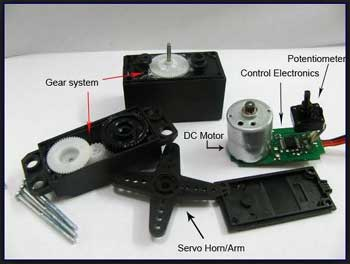
\includegraphics[scale=0.8]{sm.jpg}
	 		\centering
	 		\caption{[1]}
	 	\end{figure}
	 \textbf{PWM Principle}
	 \newline
	 It is a method to generate binary signals, which has two signal periods high and low. Depending upon the duration signal duration, power is delivered to the device.The term duty cycle is defined as:
	 \newline
	 \begin{equation}
	 	Duty Cycle = T_{ON}/(T_{ON} + T_{OFF})
	 \end{equation}
	 
	 $T_{ON}$ = On Time in one cycle \newline
	 $T_{OFF}$ = Off Time in one cycle
	 \newline
	 We use it here to control the amount of power going to the motor and hence how fast it spins.
	 
	 The diagram below shows the signal from the PWM pin of the Raspberry Pi. 
	  \begin{figure}[h!]
	  	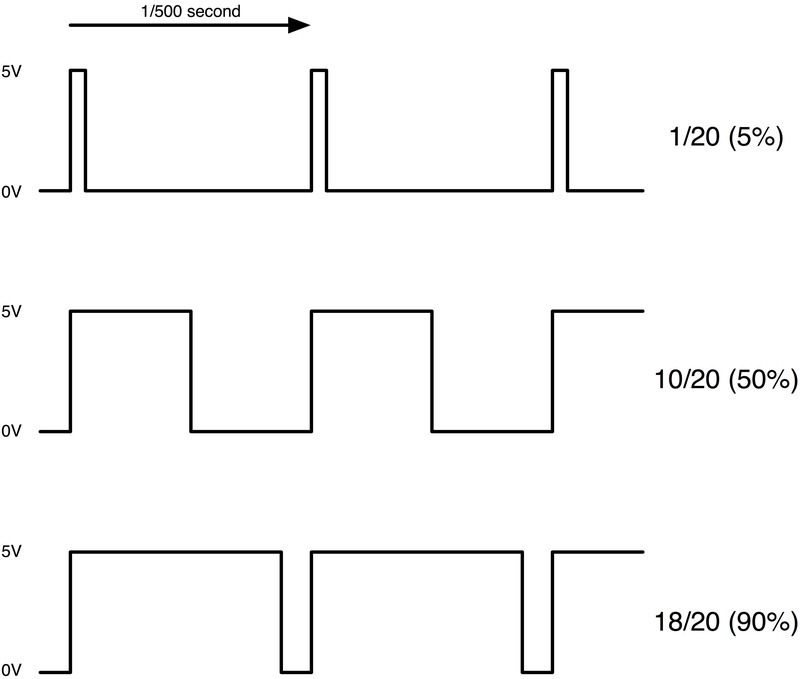
\includegraphics[scale=2.0]{pwmwaves.jpg}
	  	\centering
	  	\caption{[1]}
	  \end{figure}
	  \vspace{5mm}
	  \newline
	  Every 1/500 of a second, the PWM output will produce a pulse. The length of this pulse controls the amount of energy that the motor gets. No pulse at all and the motor will not turn, a short pulse and it will turn slowly. If the pulse is active for half the time, then the motor will receive half the power it would if the pulse stayed high until the next pulse came along.
	  \vspace{5mm}
	  \newline
	  \textbf{PCA9685 PWM Driver IC}
	   \vspace{5mm}
	  \newline
	 The PCA9685 is an I2C-bus controlled 16-channel LED controller optimized for Red/Green/Blue/Amber (RGBA) color backlighting applications. Each LED output has its own 12-bit resolution (4096 steps) fixed frequency individual PWM controller that operates at a programmable frequency from a typical of 24 Hz to 1526 Hz with a duty cycle that is
	 adjustable from  0\% to 100\% to allow the LED to be set to a specific brightness value.
	 All outputs are set to the same PWM frequency.
	 
	 We have used PCA9685 PWM servo shield given below:
	 \newline
	 \begin{figure}[h!]
	 	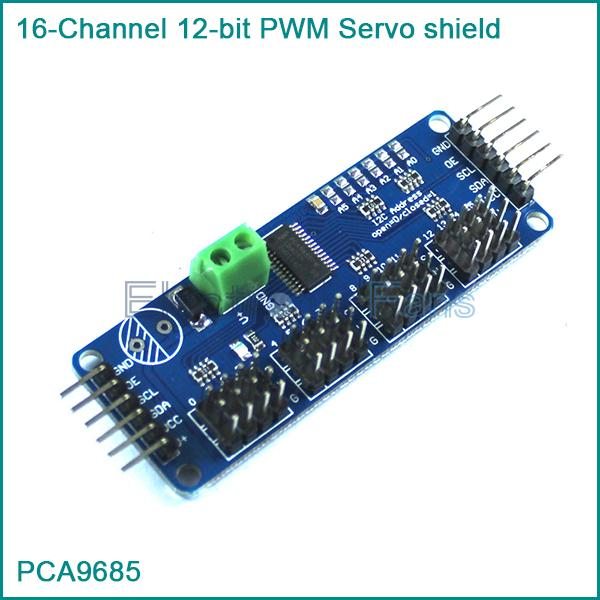
\includegraphics[scale=0.4]{pca9685.jpg}
	 	\centering
	 	\caption{[1]}
	 \end{figure}  \\
	 \newpage
	 \textbf{Pins of PCA9685 }
	 
	 \begin{figure}[h!]
	 	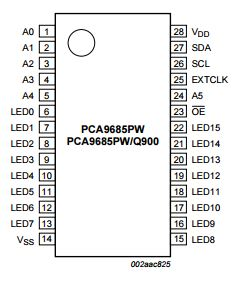
\includegraphics[scale=0.8]{pin_pca9685.jpg}
	 	\centering
	 	\caption{[1]}
	 \end{figure}
	\section{Experiment}
	
	\subsection{Controlling the speed of dc motor through L293D using PWM from the GPIO pins of RPi}  
	There is only one pin on RPi for PWM generation i.e. IC pin 12(GPIO 18).
	In this experiment we will be rotating the DC motor in both direction using L293D(Motor Driver IC) and GPIO pins of RPi.
	 
	\textbf{L293D Connections}
	\begin{center}
		\begin{tabular}{|c|c|}
			\hline
		\textbf{Pins }  & \textbf{Connections}	 \\ \hline
			
			1 & Rpi IC pin 12  \\ \hline
			2 & RPi IC pin 11  \\ \hline
			3 & motor terminal 1    \\  \hline
			4 & --		\\   \hline
			5 & -- 	\\   \hline
			6 & motor terminal 2		\\  \hline
			7 & Rpi IC pin 13		\\   \hline
			8 & Battery			\\  \hline
			13 & Battery ground		\\   \hline
			16 & 5V				\\   \hline
			
		\end{tabular}
	\end{center} 
	\vspace{1cm}
	\begin{figure}[h!]
		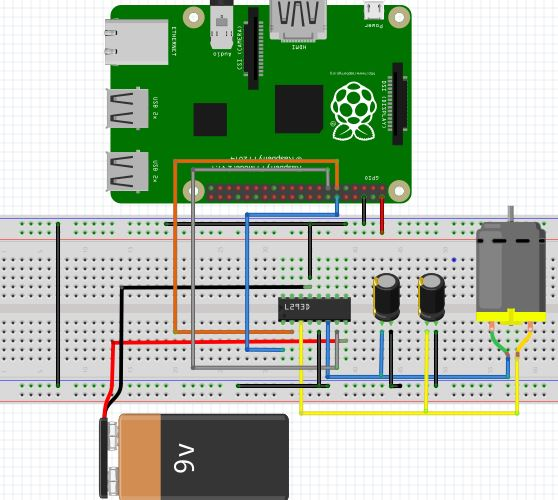
\includegraphics[scale=0.6]{DC_motor_GPIO.jpg}
		\centering
	\end{figure}

	\newpage 
	\textbf{Code}
	\vspace{0.3cm}
	\lstinputlisting[language=Python]{DC_motor_gpio.py}
	\subsection{Controlling the speed of dc motor through L293D using PWM Driver IC}
	In this experiment, we are using PWM driver IC (PCA9685) to generate PWM signal to control the velocity of dc motor.\\
	\begin{itemize}
		\item Connections to L293D is same as above except few changes listed below.
		\item Pin 1  to channel 0 of PCA9685 for PWM
		\item Pin 2 to RPi pin 11
		\item Pin 7 to Rpi pin 13 
	\end{itemize}
	\vspace{5mm}
	\begin{figure}[h!]
		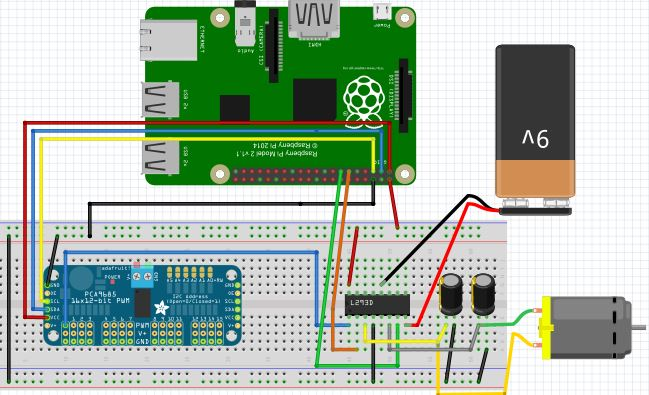
\includegraphics[scale=0.6]{DC_motor_PCA9685.jpg}
		\centering
	\end{figure} \newpage
	\textbf{Note:} Download Adafruit\_PCA9685 library from Github.\\
	\textbf{Code}
	\vspace{0.3cm}
	\lstinputlisting[language=Python]{DC_motor_PCA9685.py}
	\newpage
	
	\subsection{Controlling the velocity of servo motor using PWM Driver IC} 
	In this experiment we are using PWM driver IC(PCA9685) to generate PWM signal. \\
	\textbf{Connections}\\
	\begin{itemize}
		\item Control pin of servo motor is connected to S pin of channel 0.
		\item Ground and Vcc of servo motor is connected to ground and Vcc of channel 0 respectively.
	\end{itemize} 
	\begin{figure}[h!]
		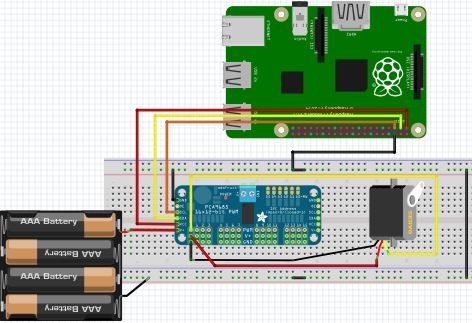
\includegraphics[scale=0.6]{servo_motor_PCA9685.jpg}
		\centering
	\end{figure}
	\vspace{5mm}

	\textbf{Note:} Download Adafruit\_PCA9685 library from Github.\\
	\textbf{Code}
	\vspace{0.3cm}
	\lstinputlisting[language=Python]{servo_PCA9685.py}
		
	\section{Exercise}
	\begin{enumerate}
			\item Interface a dc motor through L293D motor driver IC using hardware PWM pins(GPIO 18 or IC pin 12) on RPi.
	\end{enumerate}
	
	\section{Appendix}
	\subsection{PIN Diagram}
	\textbf{L293D}
	\begin{figure}[h!]
		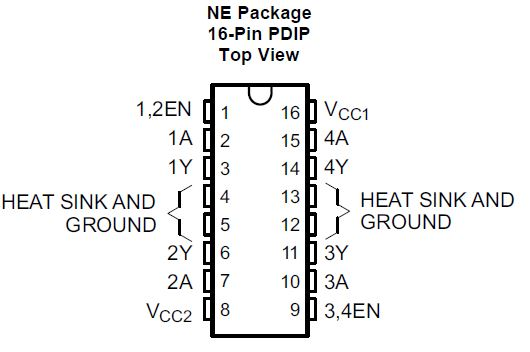
\includegraphics[scale=0.5]{l293d.jpg}
		\centering
	\end{figure} \\
	\newpage
	\textbf{MCP23017}\\
	\begin{figure}[h!]
		\includegraphics[scale=0.4]{MCP23017.png}
		\centering
	\end{figure}  
	\textbf{PCA9685}  
	\begin{figure}[h!]
		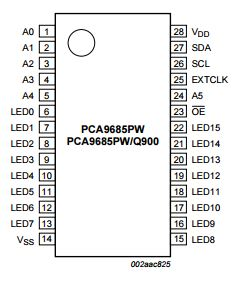
\includegraphics[scale=0.8]{pin_pca9685.jpg}
		\centering
	\end{figure} 
	\subsection{Datasheets}
	\textbf{PCA9685} \\
	\url{https://cdn-shop.adafruit.com/datasheets/PCA9685.pdf}\\
	\textbf{L293D}\\
	\url{http://www.ti.com/lit/ds/symlink/l293.pdf}
	\section{References}
	\begin{enumerate}
		\item https://projects.drogon.net/software-pwm-on-the-raspberry-pi/
		\item http://electronut.in/controlling-two-servos-with-hardware-pwm-on-the-raspberry-pi-model-a/
		\item http://raspi.tv/2013/how-to-use-soft-pwm-in-rpi-gpio-pt-2-led-dimming-and-motor-speed-control
		\item http://raspi.tv/2013/rpi-gpio-0-5-2a-now-has-software-pwm-how-to-use-it
	\end{enumerate}
	
\end{document}



